\documentclass[12pt]{article}
\usepackage[T1]{fontenc}
\usepackage[latin9]{inputenc}
\usepackage{textcomp}
\usepackage{amstext}
\usepackage{graphicx}
\usepackage{amssymb}
\makeatletter
\providecommand{\tabularnewline}{\\}

\usepackage{fourier-orns}
\usepackage[colorlinks,linkcolor=blue]{hyperref}
\usepackage{footmisc}
\usepackage{subfigure}
\usepackage{float}

\topmargin=-0.7in
\oddsidemargin = 0.2in
\parindent=0.0cm
\parskip=0.3cm
\textwidth=6.1in
\textheight= 10in

\sloppy
\newtheorem{theorem}{Theorem}[section]
\newtheorem{lemma}{Lemma}[section]
\newtheorem{corollary}{Corollary}[section]
\newtheorem{definition}{Definition}[section]


\begin{document}
{\bf Part II: }
\pagestyle{empty}

\begin{figure}[H]
  \centering
	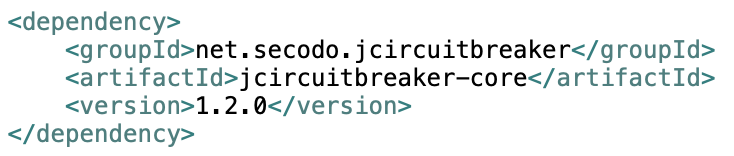
\includegraphics[width=0.6\linewidth]{code2.png}
	\caption{Add maven dependency for jcircuitbreaker-core to pom.xml}
\end{figure}

\begin{figure}[H]
  \centering
	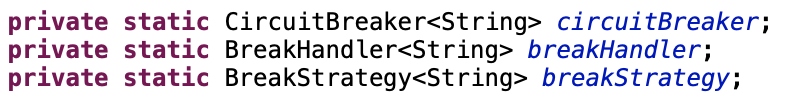
\includegraphics[width=0.6\linewidth]{code1.png}
	\caption{Prepare circuit breaker}
\end{figure}

\begin{figure}[H]
  \centering
	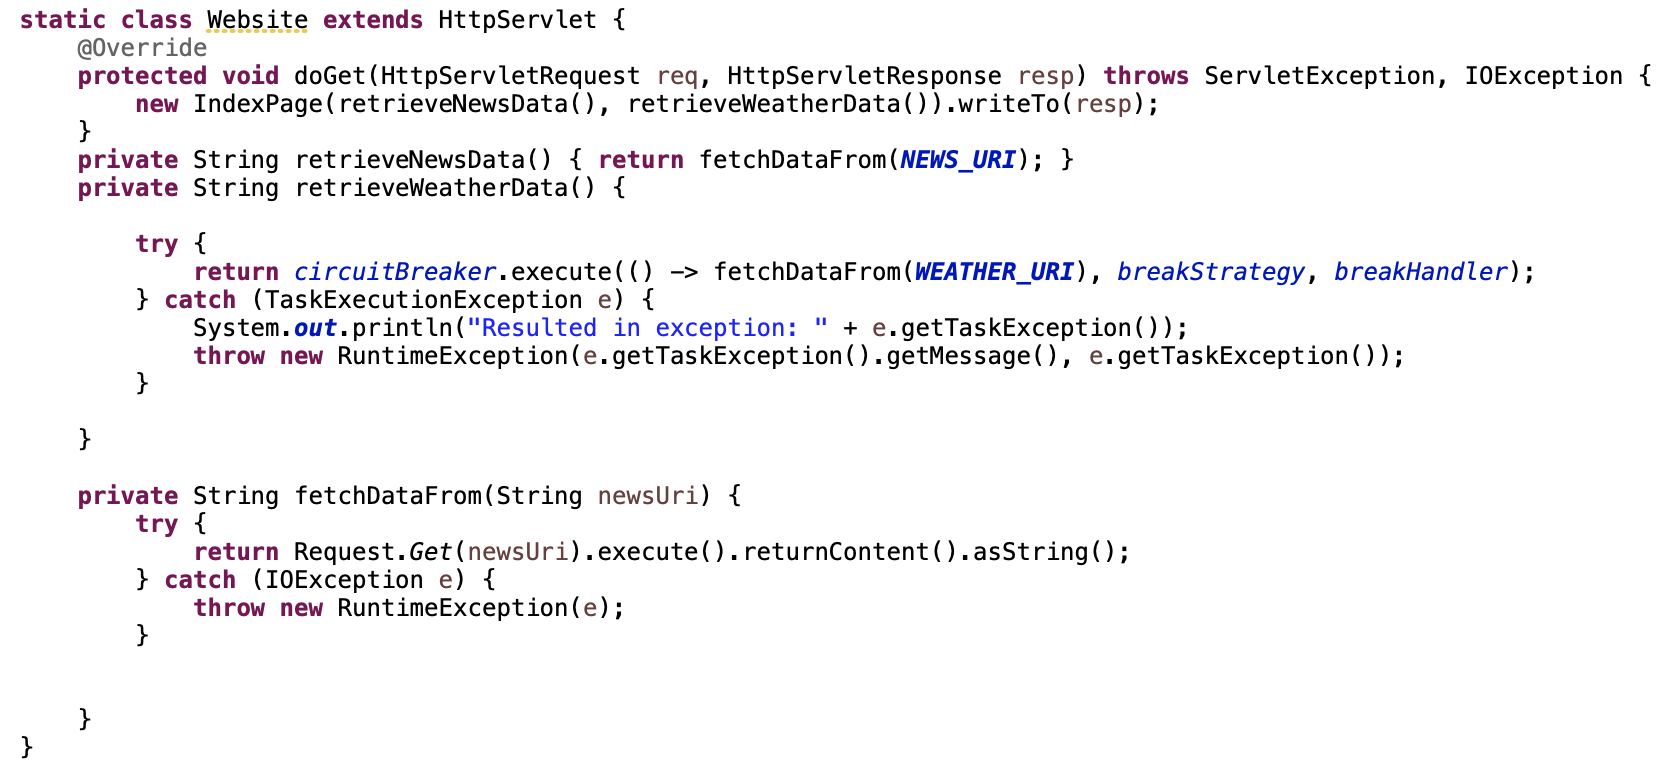
\includegraphics[width=0.8\linewidth]{code4.png}
	\caption{Replace circuit breaker for fetchDataFrom() function}
\end{figure}
If we implement the Jcircuitbreaker\footnote{http://secodo.net/projects/jcircuitbreaker/usage.html} successfully, when we open the 
front-end page: \url{http://localhost/8080/} the first time, it 
displays as lefthand side of Figure 4. Afterwards, if we refresh the page 
several times, it overloads as righthand side. It can finally display correct 
information by refreshing the page again if the overload stops. \\

\begin{figure}[H]
  \centering
	
\includegraphics[width=0.8\linewidth]{output.png}
	\caption{Left: a single request; Right: more than one requests}
\end{figure}

\end{document}